\documentclass[preprint,11pt,authoryear]{elsarticle}

\usepackage{graphicx}
\usepackage{amsmath}
\usepackage{array}
\usepackage{url}

% Plain page-number footer (no "Preprint submitted to ..." line).
\makeatletter
\def\ps@pprintTitle{%
  \let\@oddhead\@empty\let\@evenhead\@empty
  \def\@oddfoot{\hfil\thepage\hfil}\let\@evenfoot\@oddfoot}
\makeatother

\begin{document}

\begin{frontmatter}

\title{Cosmic Watch: a live, explorable observatory that applies computer vision
and machine learning to public astronomy data streams}

\author[nmims]{Jay Gupta\corref{cor}}
\ead{jay4link@gmail.com}
\cortext[cor]{ORCID: 0009-0002-7127-6146}
\affiliation[nmims]{organization={SVKM's NMIMS Mukesh Patel School of Technology
Management \& Engineering}, city={Mumbai}, country={India}}

\begin{abstract}
Public astronomy data now arrive within minutes to days of being taken, but they
are spread across many archives, formats and interfaces. We present Cosmic Watch,
an open-source Python and WebGL system that continuously collects newly released
data from thirteen public feeds (Rubin and ZTF alerts, JWST and Hubble images,
solar, space-weather, gravitational-wave, Mars rover and near-Earth-object
data), analyses it with computer vision and neural networks, cross-matches the
results against archival catalogues, and presents them in one interactive 3D
environment. On calibrated JWST imaging the source detector controls purity with
sign-flipped images and measures completeness by injecting synthetic galaxies:
on a NIRCam F460M mosaic it recovered 12,029 sources with spurious rates of
0.24\% and 0.42\% and a 5$\sigma$ point-source depth of AB 27.3. A galaxy
morphology classifier fine-tuned from Zoobot reaches 88.7\% ten-class accuracy
on Galaxy10 DECaLS, and the catalogue matcher recovers 175 of 177 reference
sources across 23 fields. We also audit the 744 anomaly candidates raised in the
first twelve days of operation, show that most were stars, long-lived active
nuclei, asteroids or relayed events, and describe vetting rules that retract
248 of 313 transient and outlier candidates. No discoveries are claimed. The
software runs on a laptop, needs no API keys, and is released under the MIT
licence.
\end{abstract}

\begin{keyword}
astronomical software \sep machine learning \sep galaxy morphology \sep
time-domain astronomy \sep source detection \sep cross-matching
\end{keyword}

\end{frontmatter}

\section{Introduction}

Most observational astronomy data are now public soon after they are taken. The
Vera C.\ Rubin Observatory \citep{Ivezic2019} and the Zwicky Transient Facility
\citep{Bellm2019} publish transient alerts in near real time through brokers
such as ALeRCE \citep{Forster2021}; new JWST and Hubble observations appear in
MAST; the Solar Dynamics Observatory \citep{Pesnell2012,Lemen2012} and
SOHO/LASCO \citep{Brueckner1995} stream solar images; and space-weather,
gravitational-wave and planetary-mission data are released through their own
services. These data are spread across many archives, formats and interfaces.
A student, educator or amateur astronomer who wants to follow the sky (what JWST
released today, whether the Sun is flaring, which transients were flagged last
night) must visit many services and has no easy way to run modern analysis on
what they find. Brokers and archive tools excel at their own data type but are
not built to put many data types side by side or to explain a result to a
non-specialist.

Cosmic Watch addresses this with one reproducible pipeline that runs on a laptop
with a consumer GPU and needs no API keys. It collects new data, analyses it with
computer vision and trained neural networks, checks the results against archival
catalogues, and presents everything in an interactive 3D environment
(Fig.~\ref{fig:app}). A design principle throughout is a clear line between
measurement and model output: for example, super-resolved pixels from SwinIR
\citep{Liang2021} or Real-ESRGAN \citep{Wang2021} are always labelled as
invented detail and never reach a detector or classifier. The system is aimed at
teaching and outreach, at student and citizen-science projects that need a
readable end-to-end example, and at quick-look triage of new releases and alerts.

This paper describes the design (Section~\ref{sec:design}), the validation of
its main components (Section~\ref{sec:validation}), an audit of the anomaly
candidates it raised in its first days of operation together with the vetting
rules that audit motivated (Section~\ref{sec:audit}), and its limitations
(Section~\ref{sec:limits}).

\begin{figure*}[t]
\centering
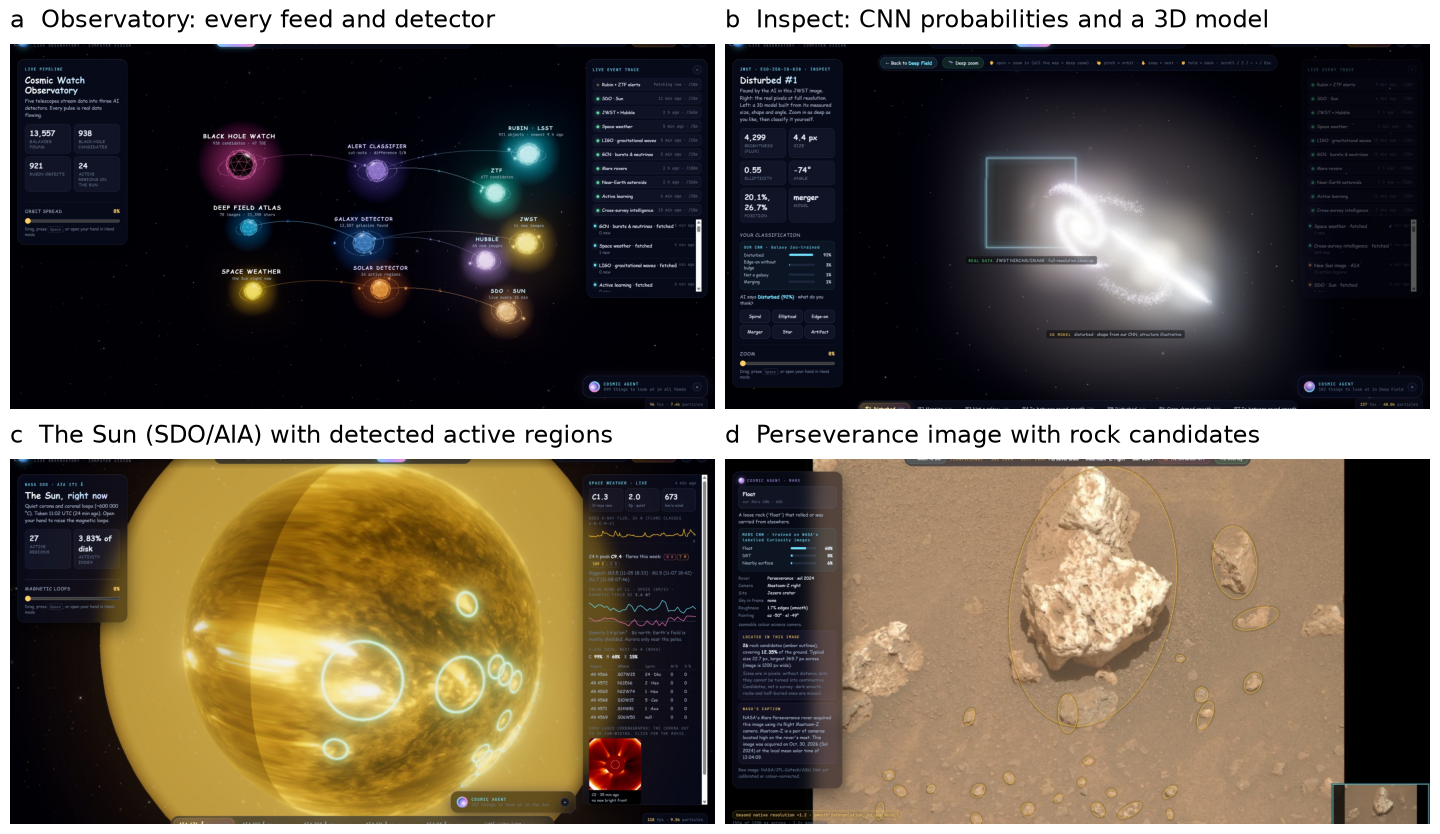
\includegraphics[width=\textwidth]{fig1_app.png}
\caption{The running application, from a live screen recording. (a) Observatory
overview: each feed and detector is a node. (b) Inspect mode for a JWST
detection: CNN probabilities beside the real pixels. (c) SDO/AIA 171\,\AA\ with
detected active regions and live NOAA space weather. (d) A Perseverance image
classified by the Mars CNN, with rock candidates outlined.}
\label{fig:app}
\end{figure*}

\section{System design}
\label{sec:design}

\subsection{Data feeds and architecture}

A FastAPI server and a scheduled pipeline write to a single SQLite database. Each
source has a fetcher and each data type a detector. The thirteen live feeds are:
Rubin and ZTF alerts via ALeRCE, new JWST and Hubble images from MAST, SDO solar
images, SOHO/LASCO coronagraph data, NOAA space-weather products,
gravitational-wave events from GraceDB, NASA GCN circulars, Mars rover images,
and NASA/JPL near-Earth-object data. Every derived claim (a classification, a
catalogue match, an anomaly flag) is stored together with the evidence that
supports it, so that any result shown to a user can be traced back to its
inputs.

\subsection{Source detection on calibrated images}

Deep-field sources are extracted with SEP \citep{Barbary2016}, the library form
of SExtractor \citep{Bertin1996}. On calibrated JWST and HST mosaics detection
runs in several passes: a cold pass for extended sources, a hot pass for compact
sources, and binned low-surface-brightness passes. Each pass is also run on the
sign-flipped image, in which any detection must be noise; detection thresholds
are raised until the spurious rate measured in this way falls below 3\%, and a
pass that cannot meet that limit is dropped. Completeness is measured by
injecting synthetic galaxies of known magnitude and size and recovering them
with the same pipeline.

\subsection{Classification models}

The galaxy classifier is a ConvNeXt-nano \citep{Liu2022} from Zoobot
\citep{Walmsley2023}, pre-trained on Galaxy Zoo DECaLS \citep{Walmsley2022} and
fine-tuned on the ten-class Galaxy10 DECaLS data set distributed with astroNN
\citep{Leung2019}. A ResNet-18 \citep{He2016} trained on the same data serves as
a baseline. Rover images are classified by a ConvNeXt-Tiny trained on the MSL
Curiosity image set of \citet{Lu2020}. Solar images are searched for sunspots,
active regions and coronal holes with classical image processing.

\subsection{Active learning}

Users can open any detection in a tiled deep-zoom view of the real pixels and
label it. These labels, together with weak labels and an eleventh
``not a galaxy'' class, are used to train challenger models. A challenger
replaces the current champion only if (i) its Galaxy10 accuracy falls by at most
1.5 percentage points, (ii) it rejects held-out stars and gas with at least 60\%
recall, and (iii) it rejects at most 10\% of held-out galaxies.

\subsection{Cross-matching}

Detections are cross-matched against Gaia DR3 \citep{Gaia2023}, Pan-STARRS1
\citep{Chambers2016}, SDSS, the DESI Legacy Imaging Surveys \citep{Dey2019} and
SIMBAD \citep{Wenger2000}. Matches are scored with a Bayesian likelihood ratio
that compares the probability of the observed separation for a true counterpart
with that for a chance alignment given the local source density, and Gaia proper
motions are applied before matching.

\subsection{Anomaly ranking and interface}

An Isolation Forest \citep{Liu2008} scores deep-field outliers, broker alerts
and cross-survey verdicts provide transient candidates, and a Thompson-sampling
bandit \citep{Thompson1933} ranks findings for the user. The front end uses
Three.js and OpenSeadragon, with optional in-browser hand-gesture control through
MediaPipe \citep{Lugaresi2019}.

\section{Validation}
\label{sec:validation}

All numbers in this section come from model cards and result files in the
repository, and a script in the repository (\texttt{paper/make\_figures.py})
rebuilds every figure from them.

\subsection{Galaxy morphology classifier}

On the 2,656-galaxy Galaxy10 validation split the classifier reaches 88.7\%
ten-class accuracy, 97.2\% top-2 accuracy and 92.7\% coarse-class accuracy,
against 82.8\%, 93.3\% and 89.5\% for the ResNet-18 baseline. The hardest classes
are \emph{Disturbed} (57\% recall) and \emph{Unbarred loose spiral} (78\%;
Fig.~\ref{fig:confusion}). Accuracy on JWST and HST imaging is expected to be
lower because of the shift in resolution, wavelength and depth from the training
images; Fig.~\ref{fig:deepfield} shows a public NIRCam image in which many small,
faint sources receive merger or disturbed labels. Of three active-learning
rounds, two challengers were correctly rejected by the promotion rules and one
was promoted, with 88.1\% Galaxy10 accuracy, 82\% recall on held-out stars and
gas, and 4.9\% of real galaxies rejected.

\begin{figure}[t]
\centering
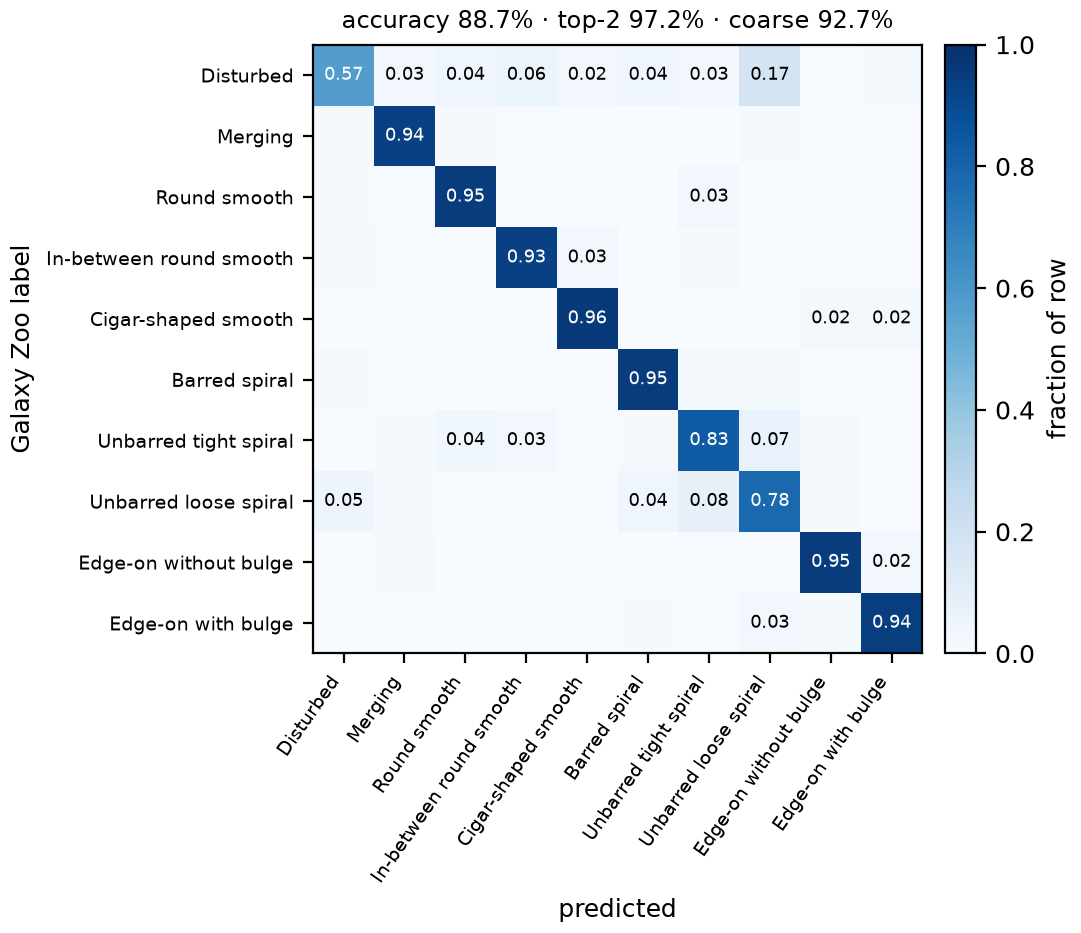
\includegraphics[width=0.85\columnwidth]{fig3_confusion.png}
\caption{Galaxy CNN confusion matrix on the Galaxy10 DECaLS validation split,
normalised by row.}
\label{fig:confusion}
\end{figure}

\begin{figure*}[t]
\centering
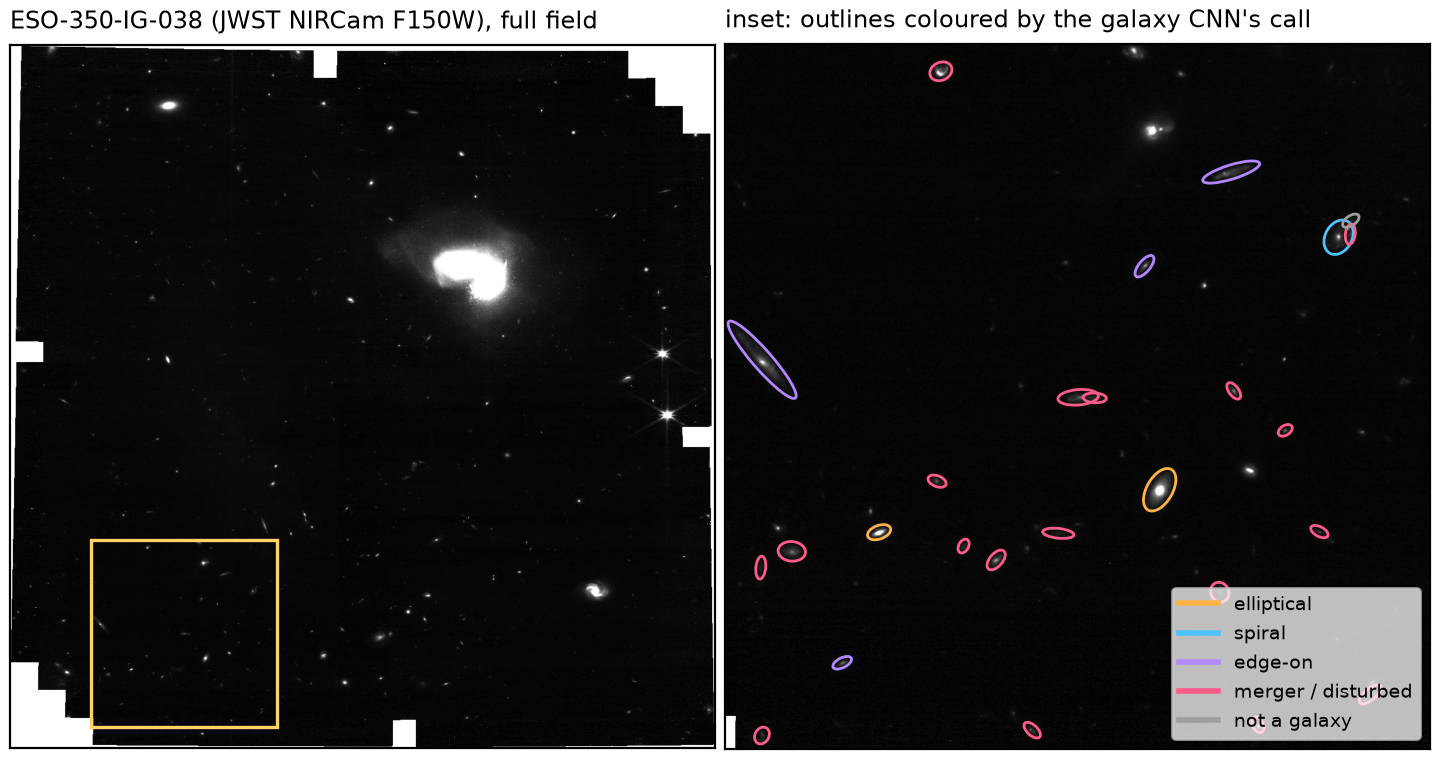
\includegraphics[width=\textwidth]{fig2_deepfield.png}
\caption{A public JWST NIRCam F150W image (ESO 350-IG038) processed by the
pipeline. Right: the boxed region with each CNN-classified detection coloured by
coarse class; the many merger/disturbed calls on small, faint sources show the
domain shift from the training images.}
\label{fig:deepfield}
\end{figure*}

\subsection{Detection on calibrated data}

On a JWST NIRCam F460M mosaic the detector found 12,029 sources, with spurious
rates measured on the sign-flipped image of 0.24\% and 0.42\% for the cold and
hot passes. The low-surface-brightness passes failed the purity test and were
dropped automatically. The 5$\sigma$ point-source depth is AB 27.3, and the 50\%
completeness limit falls from AB 25.6 for the smallest injected galaxies to
AB 21.7 for the largest (Fig.~\ref{fig:completeness}).

\begin{figure}[t]
\centering
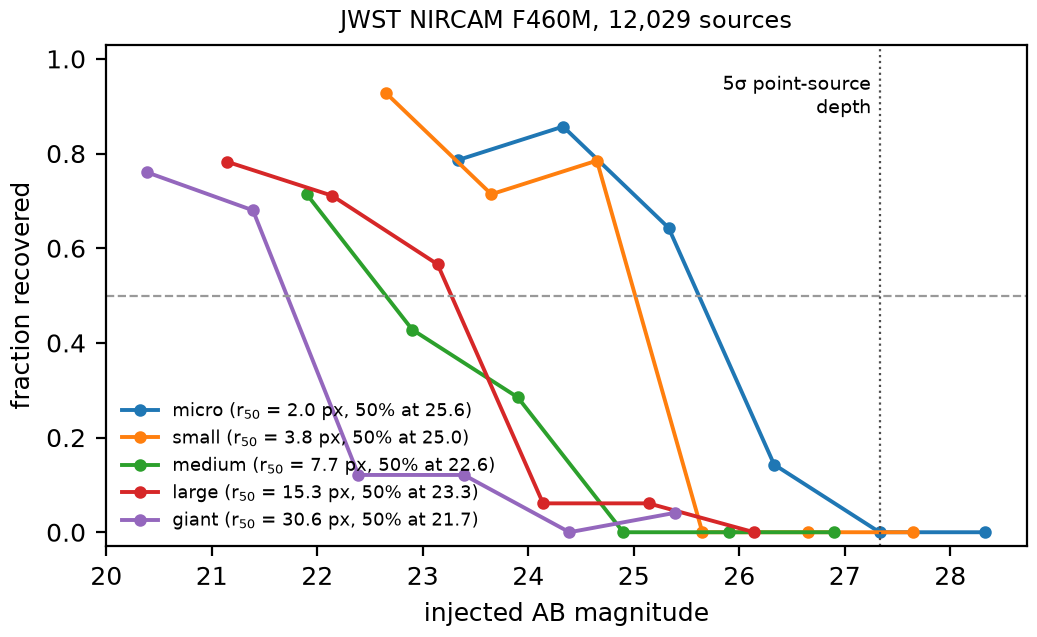
\includegraphics[width=0.9\columnwidth]{fig4_completeness.png}
\caption{Injection-recovery completeness on a calibrated JWST NIRCam F460M
mosaic, by size class (half-light radius $r_{50}$).}
\label{fig:completeness}
\end{figure}

\subsection{Cross-matching}

Using Gaia DR3's Pan-STARRS1 best-neighbour table as an answer key, the matcher
recovered 175 of 177 sources in 23 fields spanning Galactic latitudes from
$-74^\circ$ to $+76^\circ$, a precision of 98.9\% and a recall of 100\%.

\subsection{Mars terrain classifier}

The Mars classifier reaches 80.0\% accuracy (89.0\% top-3, 61.1\% balanced) on
the test split of \citet{Lu2020}, which uses sols not seen in training.

\section{Operation and audit of anomaly candidates}
\label{sec:audit}

In its first twelve days of operation (30 October to 10 November 2026) the
pipeline ingested 824 images, 1,870 Rubin and ZTF alerts and 46,455 detections,
built 3,857 cross-survey objects from 29,191 archive matches, and raised 744
candidate anomalies.

These candidates are not discoveries, and an audit of them shows why
(Table~\ref{tab:audit}). Only 394 concern individual astronomical objects; the
rest are solar-activity changes or relays of events announced by other
facilities, and only 56 (7.5\%) had been reviewed by a person. Of the 211
deep-field outliers, 96 are point sources and 26 more are rejected by the CNN as
``not a galaxy'', so the Isolation Forest mostly selected the brightest and
largest sources. Of 29 broker tidal-disruption candidates, 23 were first
detected two or more years earlier, which a flare lasting months cannot explain.
Half of the ``hostless'' transients (8 of 16) are single-detection alerts that
the broker classes as asteroids, and 29 of 57 supernova candidates carry an AGN,
QSO or blazar class.

We therefore added vetting rules, implemented in one module with unit tests and
shared by the live pipeline and the re-measurement: deep-field ``normal'' is
defined over extended sources only; tidal-disruption candidates must be young
and not identified as stars or AGN by the archives; a ``new, hostless'' verdict
needs repeat detections, a successful check against known asteroids using JPL
ephemerides, and a recent first detection; and supernova candidates must not
carry an AGN-type broker class. Re-applied to the same data
(Table~\ref{tab:audit}), the rules retracted 248 of 313 transient and outlier
candidates. In a visual inspection of 24 randomly chosen outliers before and
after vetting, the fraction that were real galaxies rose from 9 of 24 to 14 of
24; the remaining contaminants are nebulae, satellite trails and detector
artefacts. None of the surviving candidates has yet been confirmed as
scientifically unusual. The next steps are adjudication against spectroscopic
classifications from the Transient Name Server and a measured precision on a
larger, independently vetted sample.

\begin{table*}[t]
\centering
\caption{Anomaly candidates raised from 30 October to 10 November 2026, before
and after the vetting rules.}
\label{tab:audit}
\small
\begin{tabular}{>{\raggedright\arraybackslash}p{3.3cm}r>{\raggedright\arraybackslash}p{2.1cm}>{\raggedright\arraybackslash}p{4.3cm}}
\hline
Candidate type & Raised & After vetting & Main reason for retraction \\
\hline
Deep-field outliers & 211 & 33 (+51 newly selected) & star (96), CNN ``not a galaxy'' (28) \\
Tidal-disruption candidates & 29 & 4 & first detected years earlier (23) \\
Supernova candidates & 57 & 28 & broker class AGN/QSO/blazar (29) \\
``New, hostless'' transients & 16 & 0 & broker asteroid (8), not new (6) \\
CNN mergers, nuclear transients & 81 & 81 & not yet vetted \\
Solar, relayed and other events & 350 & 350 & not object discovery \\
\hline
\textbf{Total} & \textbf{744} & \textbf{496 + 51} & 56 had been reviewed by a person \\
\hline
\end{tabular}
\end{table*}

\section{Limitations}
\label{sec:limits}

Classifications are probabilistic, and on JWST and HST data they are applied
outside the training domain. Detections made on preview (non-calibrated) images
are indicative only. Rubin full frames are not public in real time, so Rubin
coverage is limited to alerts. The anomaly candidates have not been validated
against spectroscopic classifications. Cosmic Watch complements, and does not
replace, the archives and brokers it draws on.

\section{Conclusions}

Cosmic Watch brings thirteen public astronomy data streams into one pipeline and
one interactive environment, with measured purity and completeness on calibrated
JWST data, a validated galaxy classifier and catalogue matcher, and an
evidence trail for every claim. Its first days of operation also show that an
unvetted anomaly stream is dominated by stars, long-lived active nuclei,
asteroids and relayed events, and that simple, tested vetting rules remove most
of them. The code, model cards and figure scripts are public so that every
number in this paper can be reproduced.

\section*{Code availability}

The source code is available under the MIT licence at\\
\url{https://github.com/jay4linkh/cosmic-watch-ai}.

\section*{AI usage disclosure}

Generative AI was used in this work. Anthropic's Claude (Claude Opus models,
accessed through the Claude Code assistant in 2026) was used to help write,
refactor and test parts of the software and its documentation, and to help
draft and edit this manuscript. The author designed the system and chose the
methods, ran every experiment, checked every number reported here against the
repository's result files, and reviewed, modified and validated all
AI-assisted code and text. The author takes full responsibility for the
content of this paper.

\section*{Acknowledgements}

This work uses public data and services from NASA, ESA, STScI/MAST, the Vera C.\
Rubin Observatory, ZTF and ALeRCE, LIGO, Virgo and KAGRA via GraceDB, NASA GCN,
NASA/SDO and the AIA and HMI teams, SOHO/LASCO, NOAA SWPC, NASA/JPL-Caltech,
SDSS, Pan-STARRS, ESA Gaia, CDS/SIMBAD, NED, the DESI Legacy Imaging Surveys and
the NOIRLab Astro Data Lab, and builds on Zoobot and the Galaxy Zoo volunteers.
This project is dedicated to the author's late mother.

\bibliographystyle{elsarticle-harv}
\bibliography{cosmic-watch}

\end{document}
